\section{Theoretical Analysis}
\label{sec:analysis}

In this section are shown the obtained results using a suitable theoretical model able to predict the output of the Envelope Detector and voltage Regulator circuits.
The theoretical output is calculated using an octave script. Within this script are used both Kirchoff's Laws and diodes equations as well as simplified models of the two. 

\subsection{Envelope detector}
The main goal of an envelope detector is to restrict the voltage's amplitude. Different from the voltage regulator that decreases the ripple. As it was shown in the circuit's figure, the envelope detector is, basically, the resistance and the capacitor in parallel. Its main function is to decrease the ripple using the following expression:\par
\begin{equation}
    v_0(t) = Acos(\omega t_{off})^{\frac{-t+t_{off}}{RC}}
\end{equation}\par
Where: \par
\begin{itemize}
  \item A - Amplitude
  \item $\omega$ - angular frequency
  \item R - Resistance, constant obtained using the following expression:
\end{itemize}
\begin{equation}
    R = R_3 + 23r_d 
\end{equation}\par
$R_3$ and $r_d$ will be explained in the next section.\par
\begin{itemize}
  \item C - Capacitance
  \item $t_{off}$ - Constant obtained using the following expression:
\end{itemize}
\begin{equation}
    t_{off}=\frac{1}{\omega}arctan(\frac{1}{\omega RC})
\end{equation}\par

\begin{figure}[H] \centering
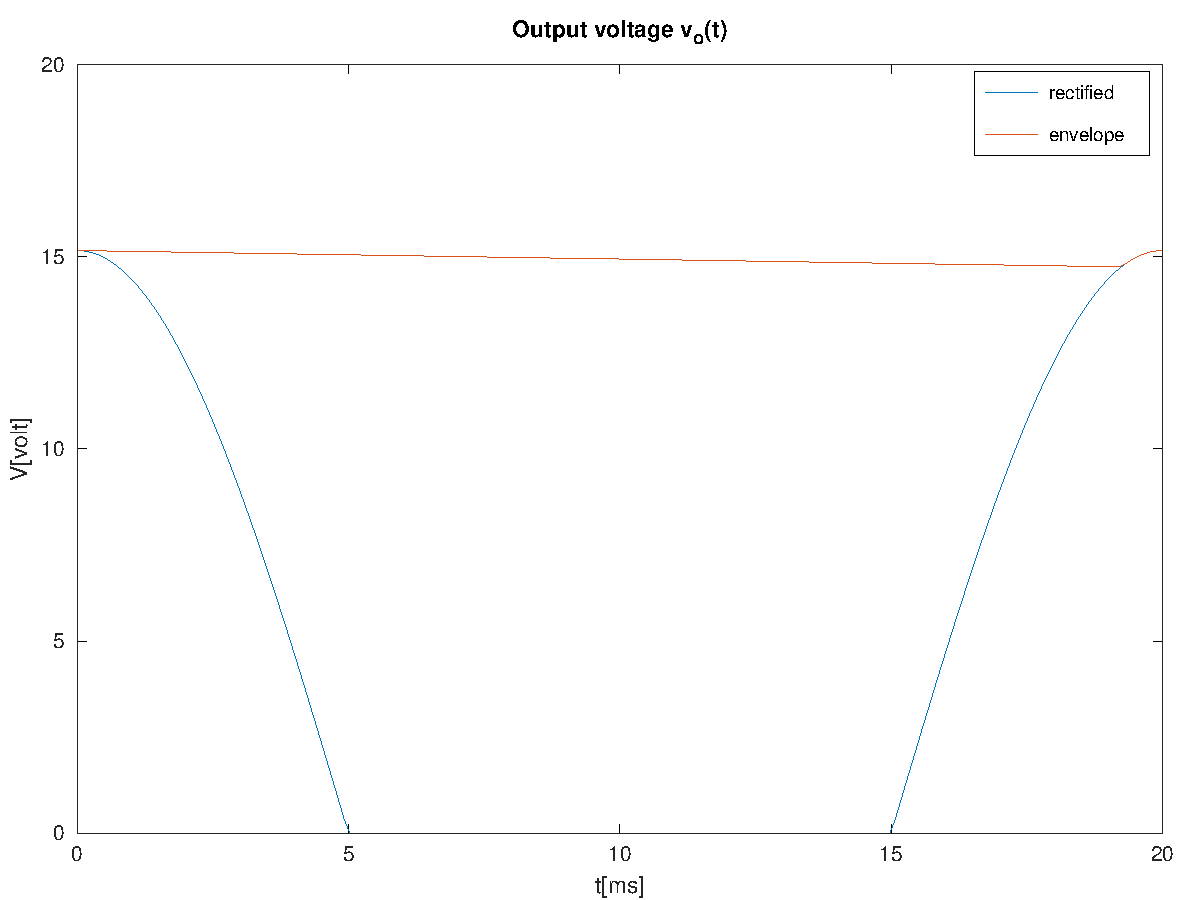
\includegraphics[width=0.7\linewidth]{../mat/retified.pdf}
\caption{Rectified Signal.}
\label{fig:rectified}
\end{figure}

\begin{figure}[H] \centering
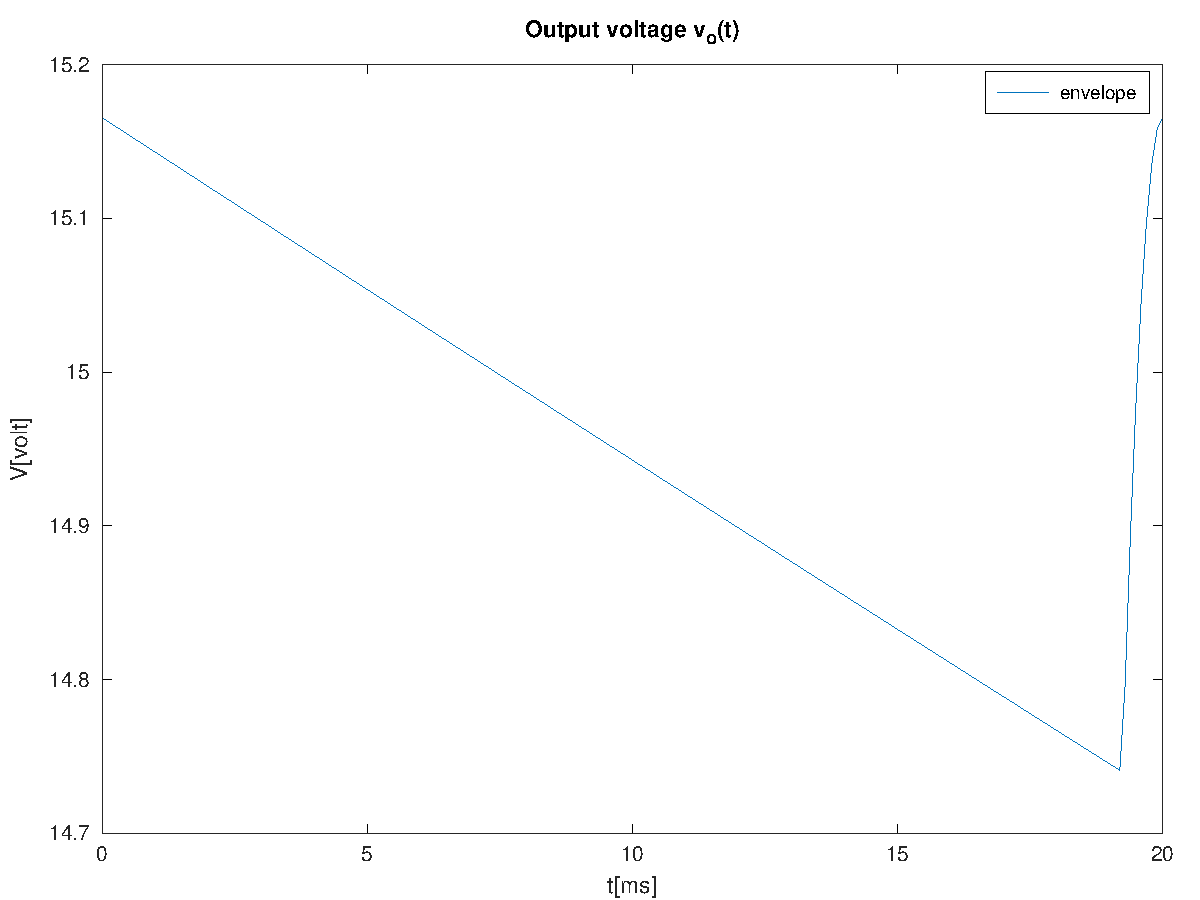
\includegraphics[width=0.7\linewidth]{../mat/envelope.pdf}
\caption{Envelope Detector Output Voltage.}
\label{fig:envelopeth}
\end{figure}

\subsection{Voltage Regulator}
In our circuit, the voltage regulator consists of 19 diodes in series that will impose the 12V voltage. The resistance in series will decrease the amplitude.\par
The expressions used to do this were the following ones:\par
Sinusoidal part from envelope:\par
\begin{equation}
    v_{sr} = v_O - V_s
\end{equation}\par
Calculating $rd_{n}$ for all the diodes, where $rd$ is the resistance of each one:\par
\begin{equation}
    rd_n = 23rd
\end{equation}\par
And then, we have: \par
\begin{equation}
    vO_r = (\frac{rd_n}{rd_n + R_3})v_{sr}
\end{equation}\par
Where $R_3$ is the resistance in serie.\par
The expression used to obtain the vltage ripple was: \par
\begin{equation}
    v_{ripple} = maximum(V_{dc})-minimum(V_{dc})
\end{equation}\par
Where: \par
\begin{equation}
    V_{dc} = 21V_{on} + vO_r
\end{equation}\par
The results are shown below:\par

\begin{figure}[H] \centering
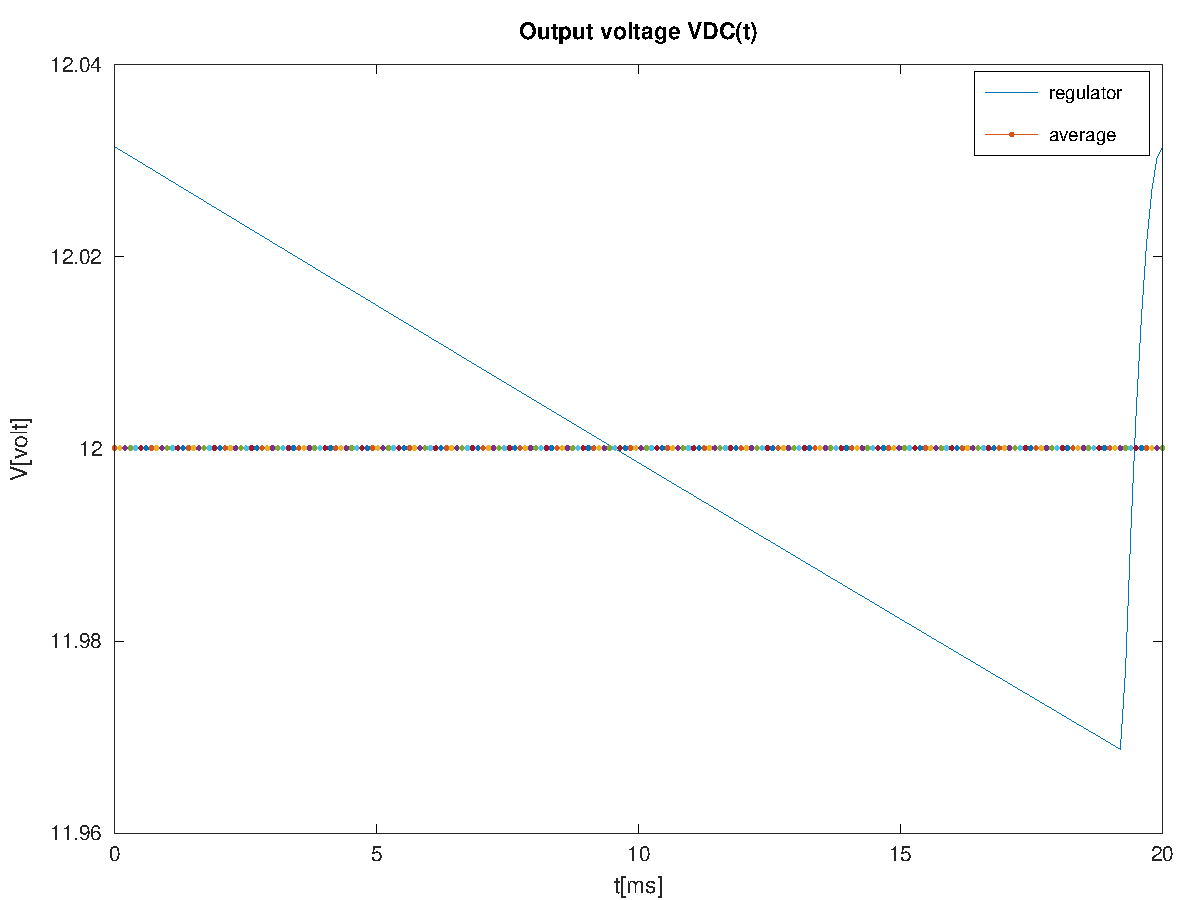
\includegraphics[width=0.7\linewidth]{../mat/outputdc.pdf}
\caption{DC Output Signal.}
\label{fig:outputdc}
\end{figure}

\begin{figure}[H] \centering
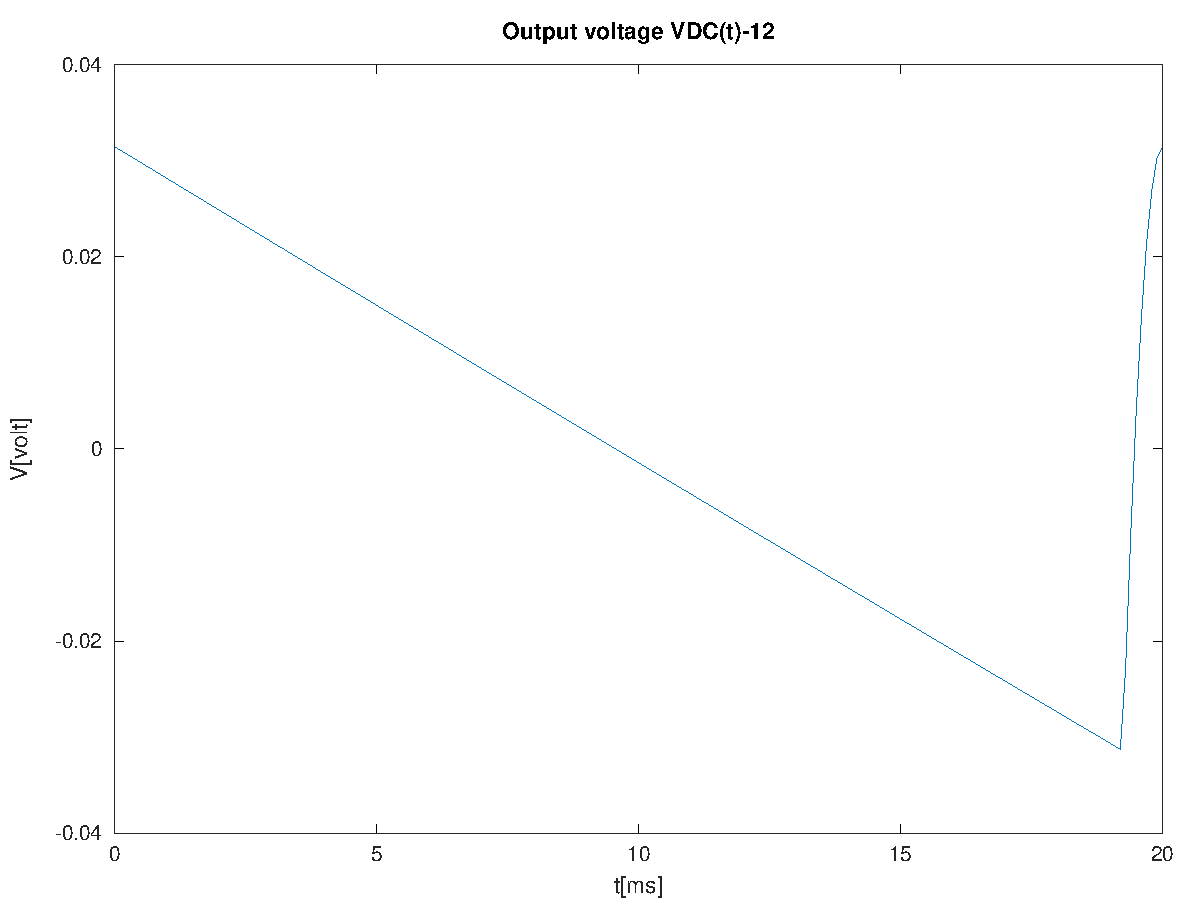
\includegraphics[width=0.7\linewidth]{../mat/v012.pdf}
\caption{Output Signal - 12 (deviation).}
\label{fig:v012}
\end{figure}

\begin{table}[H]
  \centering
  \begin{tabular}{|l|r|}
    \hline    
    {\bf Name} & {\bf Value [V]} \\ \hline
    \input{../mat/ripple_octave}
  \end{tabular}
  \label{tab:ripple}
\end{table}

\begin{figure}[H] \centering
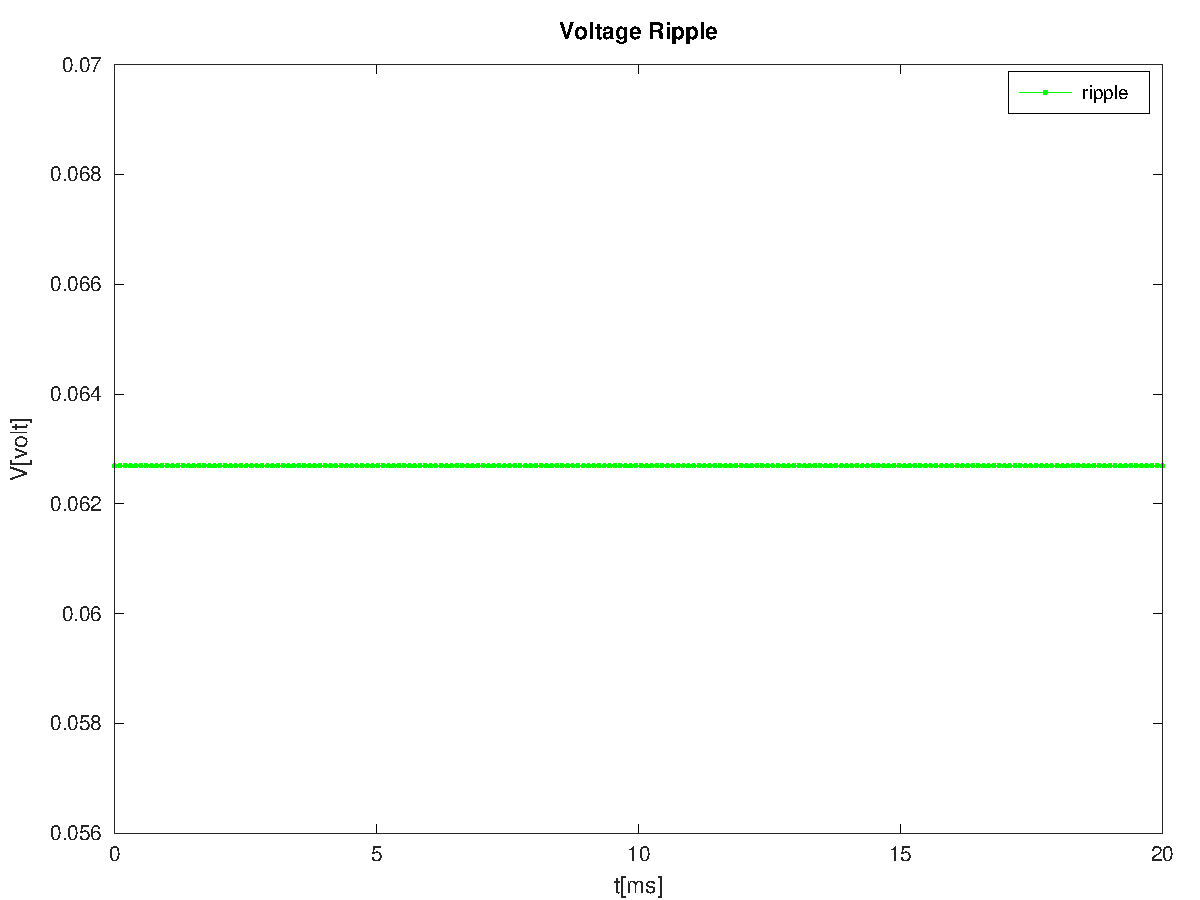
\includegraphics[width=0.7\linewidth]{../mat/ripple.pdf}
\caption{Ripple.}
\label{fig:ripplegraph}
\end{figure}